
We can calculate the t dependence of the differential cross section $d\sigma_U/dt$ by integrating the reduced cross sections over $\phi$ as in equation \ref{eq:tdep}

 \begin{equation}\label{eq:tdep}
    \frac{d\sigma_U}{dt} = \int \frac{d^2\sigma}{dtd\phi} d\phi
\end{equation}

In order to account for regions where the detectors used in CLAS6 and CLAS12 have zero acceptance, it is necessary to include a correction factor $\eta'$, defined in equation \ref{eq:eta} and calculated using Monte Carlo. 

 \begin{equation}\label{eq:eta}
    \eta' = \frac{\int_{\Omega*} \frac{d^2\sigma}{dtd\phi} }{\int_{\Omega} \frac{d^2\sigma}{dtd\phi}}
\end{equation}

However, at this point this correction factor has not yet been calculated. Instead, we can focus on kinematic bins where the coverage in $\phi$ is nearly 100\%, such that $\eta'$ would be small. In figure \ref{fig:tdep} we show the t dependent cross section, calculated only for bins where the coverage in $\phi$ was greater than 90\%, thus the error from not including the $\eta'$ correction factor is only approximately 10\%. We observe a good agreement in the b slope parameter, which describes the width of the transverse momentum distribution of the proton, between CLAS12 and the published CLAS6 data.


\begin{figure}[hbt]
	\centering
	\includegraphics[page=125,width=0.45\linewidth]{Chapters/Ch5-Further/t_dependence/pics/fig_1.0_0.15.png}
	\includegraphics[page=130,width=0.45\linewidth]{Chapters/Ch5-Further/t_dependence/pics/fig_1.5_0.15.png}

	\caption[t dependence]{CLAS12 and CLAS6 t dependence of cross sections. The fits are exponential functions $Ae^{-bt}$, where the slope parameter b are in close agreement for the bins considered. The overall normalization A is not yet determined for the CLAS12 dataset, so a small overall offset from the CLAS6 data is expected. Errors are only statistical.}
	\label{fig:tdep}
\end{figure}


\begin{figure}[hbt]
	\centering
	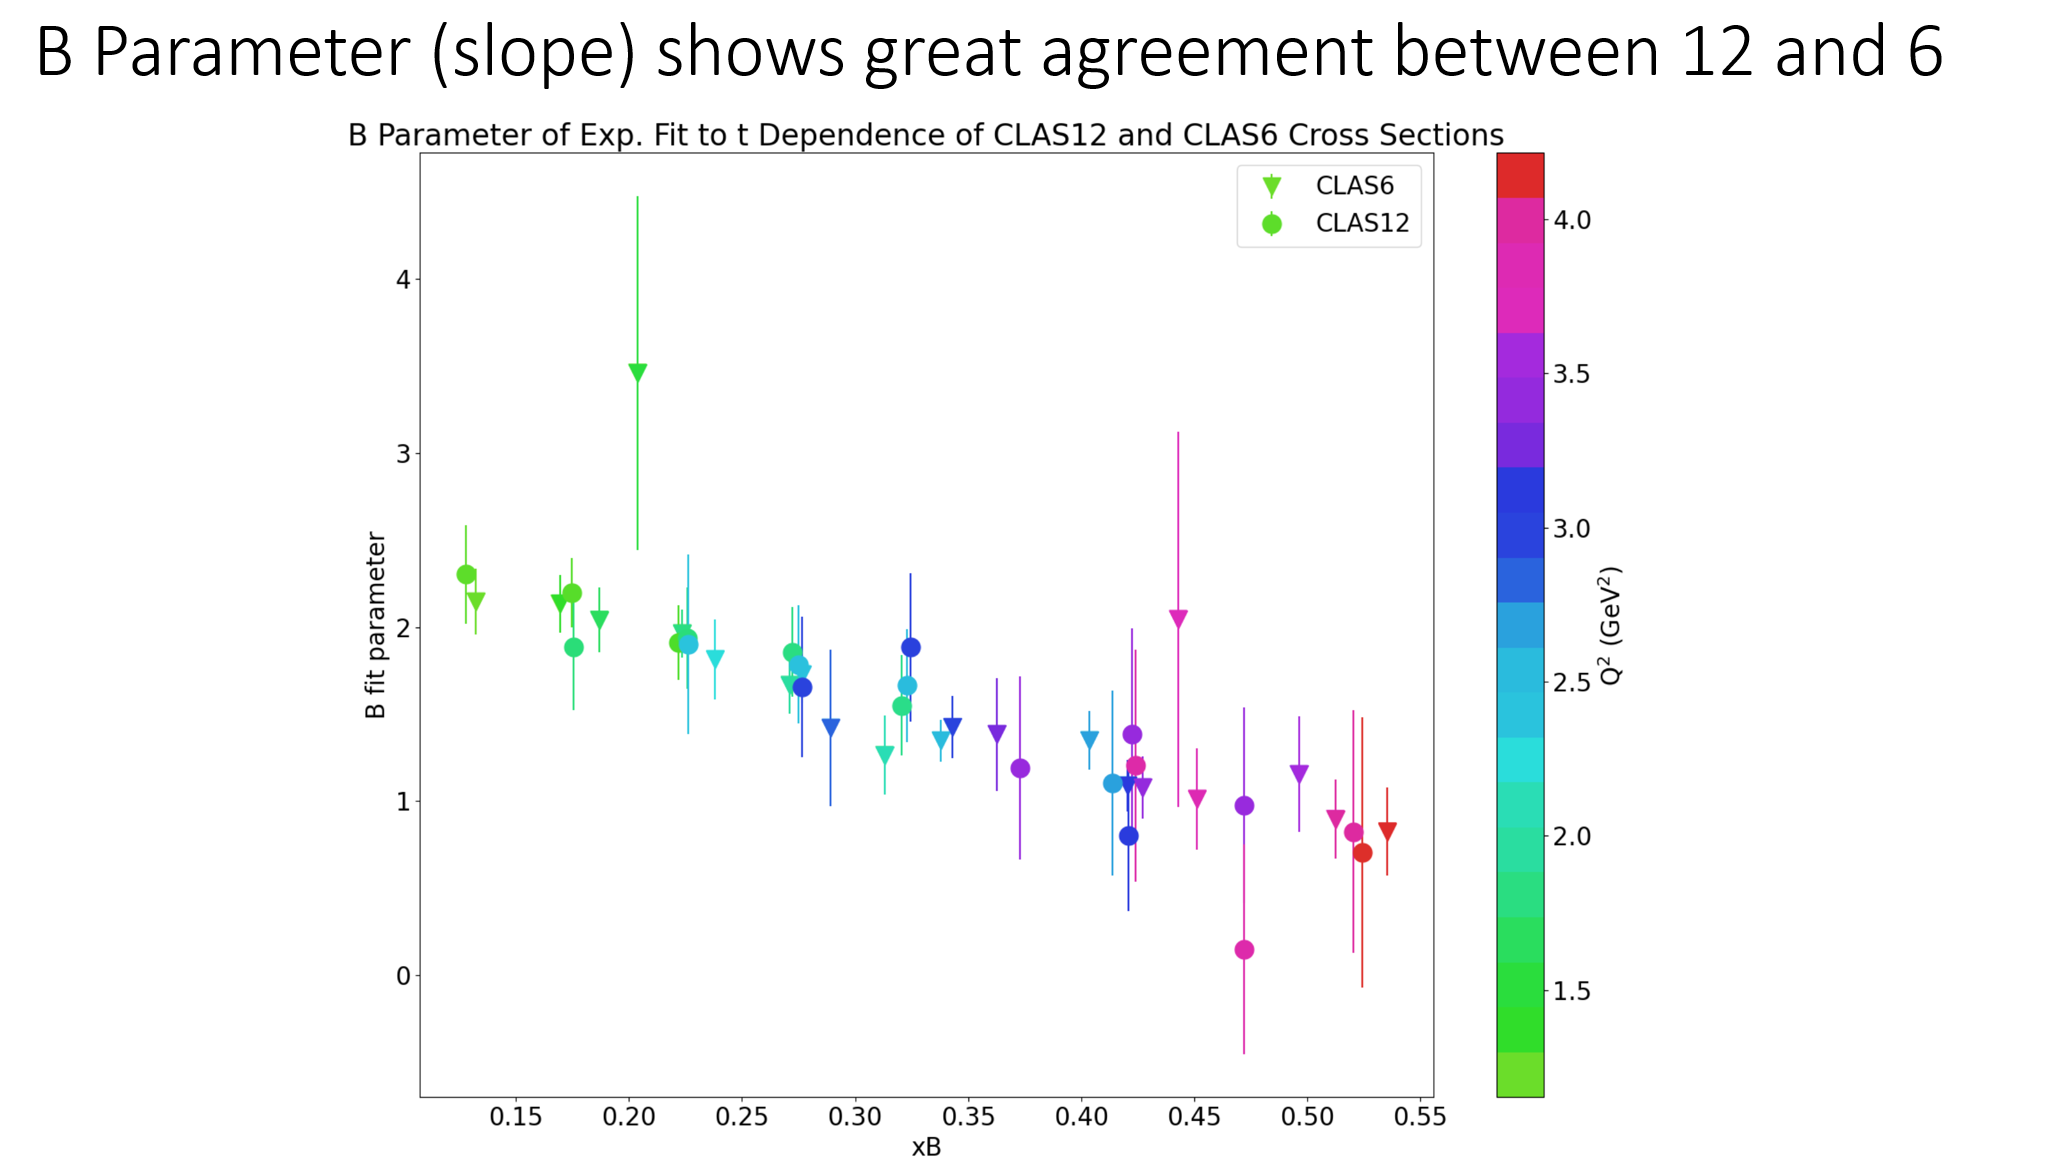
\includegraphics[trim={0 0 0 2.2cm},clip,width=0.8\linewidth]{Chapters/Ch5-Further/t_dependence/pics/bslopes.png}

	\caption[Bslopes]{CLAS12 and CLAS6 t dependence of cross sections. The fits are exponential functions $Ae^{-bt}$, where the slope parameter b are in close agreement for the bins considered. The overall normalization A is not yet determined for the CLAS12 dataset, so a small overall offset from the CLAS6 data is expected. Errors are only statistical.}
	\label{fig:bslopes}
\end{figure}
